% Options for packages loaded elsewhere
\PassOptionsToPackage{unicode}{hyperref}
\PassOptionsToPackage{hyphens}{url}
%
\documentclass[
]{article}
\usepackage{amsmath,amssymb}
\usepackage{lmodern}
\usepackage{iftex}
\ifPDFTeX
  \usepackage[T1]{fontenc}
  \usepackage[utf8]{inputenc}
  \usepackage{textcomp} % provide euro and other symbols
\else % if luatex or xetex
  \usepackage{unicode-math}
  \defaultfontfeatures{Scale=MatchLowercase}
  \defaultfontfeatures[\rmfamily]{Ligatures=TeX,Scale=1}
\fi
% Use upquote if available, for straight quotes in verbatim environments
\IfFileExists{upquote.sty}{\usepackage{upquote}}{}
\IfFileExists{microtype.sty}{% use microtype if available
  \usepackage[]{microtype}
  \UseMicrotypeSet[protrusion]{basicmath} % disable protrusion for tt fonts
}{}
\makeatletter
\@ifundefined{KOMAClassName}{% if non-KOMA class
  \IfFileExists{parskip.sty}{%
    \usepackage{parskip}
  }{% else
    \setlength{\parindent}{0pt}
    \setlength{\parskip}{6pt plus 2pt minus 1pt}}
}{% if KOMA class
  \KOMAoptions{parskip=half}}
\makeatother
\usepackage{xcolor}
\usepackage[margin=1in]{geometry}
\usepackage{longtable,booktabs,array}
\usepackage{calc} % for calculating minipage widths
% Correct order of tables after \paragraph or \subparagraph
\usepackage{etoolbox}
\makeatletter
\patchcmd\longtable{\par}{\if@noskipsec\mbox{}\fi\par}{}{}
\makeatother
% Allow footnotes in longtable head/foot
\IfFileExists{footnotehyper.sty}{\usepackage{footnotehyper}}{\usepackage{footnote}}
\makesavenoteenv{longtable}
\usepackage{graphicx}
\makeatletter
\def\maxwidth{\ifdim\Gin@nat@width>\linewidth\linewidth\else\Gin@nat@width\fi}
\def\maxheight{\ifdim\Gin@nat@height>\textheight\textheight\else\Gin@nat@height\fi}
\makeatother
% Scale images if necessary, so that they will not overflow the page
% margins by default, and it is still possible to overwrite the defaults
% using explicit options in \includegraphics[width, height, ...]{}
\setkeys{Gin}{width=\maxwidth,height=\maxheight,keepaspectratio}
% Set default figure placement to htbp
\makeatletter
\def\fps@figure{htbp}
\makeatother
\setlength{\emergencystretch}{3em} % prevent overfull lines
\providecommand{\tightlist}{%
  \setlength{\itemsep}{0pt}\setlength{\parskip}{0pt}}
\setcounter{secnumdepth}{-\maxdimen} % remove section numbering
\ifLuaTeX
  \usepackage{selnolig}  % disable illegal ligatures
\fi
\IfFileExists{bookmark.sty}{\usepackage{bookmark}}{\usepackage{hyperref}}
\IfFileExists{xurl.sty}{\usepackage{xurl}}{} % add URL line breaks if available
\urlstyle{same} % disable monospaced font for URLs
\hypersetup{
  pdftitle={Books\_ratings},
  pdfauthor={Christophe},
  hidelinks,
  pdfcreator={LaTeX via pandoc}}

\title{Books\_ratings}
\author{Christophe}
\date{}

\begin{document}
\maketitle

{
\setcounter{tocdepth}{2}
\tableofcontents
}
data inspection

\begin{longtable}[]{@{}ll@{}}
\caption{Data summary}\tabularnewline
\toprule()
\endhead
Name & data \\
Number of rows & 11127 \\
Number of columns & 12 \\
\_\_\_\_\_\_\_\_\_\_\_\_\_\_\_\_\_\_\_\_\_\_\_ & \\
Column type frequency: & \\
character & 7 \\
numeric & 5 \\
\_\_\_\_\_\_\_\_\_\_\_\_\_\_\_\_\_\_\_\_\_\_\_\_ & \\
Group variables & None \\
\bottomrule()
\end{longtable}

\textbf{Variable type: character}

\begin{longtable}[]{@{}
  >{\raggedright\arraybackslash}p{(\columnwidth - 14\tabcolsep) * \real{0.2267}}
  >{\raggedleft\arraybackslash}p{(\columnwidth - 14\tabcolsep) * \real{0.1333}}
  >{\raggedleft\arraybackslash}p{(\columnwidth - 14\tabcolsep) * \real{0.1867}}
  >{\raggedleft\arraybackslash}p{(\columnwidth - 14\tabcolsep) * \real{0.0533}}
  >{\raggedleft\arraybackslash}p{(\columnwidth - 14\tabcolsep) * \real{0.0533}}
  >{\raggedleft\arraybackslash}p{(\columnwidth - 14\tabcolsep) * \real{0.0800}}
  >{\raggedleft\arraybackslash}p{(\columnwidth - 14\tabcolsep) * \real{0.1200}}
  >{\raggedleft\arraybackslash}p{(\columnwidth - 14\tabcolsep) * \real{0.1467}}@{}}
\toprule()
\begin{minipage}[b]{\linewidth}\raggedright
skim\_variable
\end{minipage} & \begin{minipage}[b]{\linewidth}\raggedleft
n\_missing
\end{minipage} & \begin{minipage}[b]{\linewidth}\raggedleft
complete\_rate
\end{minipage} & \begin{minipage}[b]{\linewidth}\raggedleft
min
\end{minipage} & \begin{minipage}[b]{\linewidth}\raggedleft
max
\end{minipage} & \begin{minipage}[b]{\linewidth}\raggedleft
empty
\end{minipage} & \begin{minipage}[b]{\linewidth}\raggedleft
n\_unique
\end{minipage} & \begin{minipage}[b]{\linewidth}\raggedleft
whitespace
\end{minipage} \\
\midrule()
\endhead
title & 0 & 1 & 2 & 254 & 0 & 10352 & 0 \\
authors & 0 & 1 & 3 & 750 & 0 & 6643 & 0 \\
isbn & 0 & 1 & 9 & 10 & 0 & 11127 & 0 \\
isbn13 & 0 & 1 & 13 & 13 & 0 & 11127 & 0 \\
language\_code & 0 & 1 & 2 & 5 & 0 & 27 & 0 \\
publication\_date & 0 & 1 & 8 & 10 & 0 & 3679 & 0 \\
publisher & 0 & 1 & 2 & 67 & 0 & 2292 & 0 \\
\bottomrule()
\end{longtable}

\textbf{Variable type: numeric}

\begin{longtable}[]{@{}
  >{\raggedright\arraybackslash}p{(\columnwidth - 20\tabcolsep) * \real{0.1792}}
  >{\raggedleft\arraybackslash}p{(\columnwidth - 20\tabcolsep) * \real{0.0943}}
  >{\raggedleft\arraybackslash}p{(\columnwidth - 20\tabcolsep) * \real{0.1321}}
  >{\raggedleft\arraybackslash}p{(\columnwidth - 20\tabcolsep) * \real{0.0849}}
  >{\raggedleft\arraybackslash}p{(\columnwidth - 20\tabcolsep) * \real{0.0943}}
  >{\raggedleft\arraybackslash}p{(\columnwidth - 20\tabcolsep) * \real{0.0283}}
  >{\raggedleft\arraybackslash}p{(\columnwidth - 20\tabcolsep) * \real{0.0849}}
  >{\raggedleft\arraybackslash}p{(\columnwidth - 20\tabcolsep) * \real{0.0849}}
  >{\raggedleft\arraybackslash}p{(\columnwidth - 20\tabcolsep) * \real{0.0849}}
  >{\raggedleft\arraybackslash}p{(\columnwidth - 20\tabcolsep) * \real{0.0755}}
  >{\raggedright\arraybackslash}p{(\columnwidth - 20\tabcolsep) * \real{0.0566}}@{}}
\toprule()
\begin{minipage}[b]{\linewidth}\raggedright
skim\_variable
\end{minipage} & \begin{minipage}[b]{\linewidth}\raggedleft
n\_missing
\end{minipage} & \begin{minipage}[b]{\linewidth}\raggedleft
complete\_rate
\end{minipage} & \begin{minipage}[b]{\linewidth}\raggedleft
mean
\end{minipage} & \begin{minipage}[b]{\linewidth}\raggedleft
sd
\end{minipage} & \begin{minipage}[b]{\linewidth}\raggedleft
p0
\end{minipage} & \begin{minipage}[b]{\linewidth}\raggedleft
p25
\end{minipage} & \begin{minipage}[b]{\linewidth}\raggedleft
p50
\end{minipage} & \begin{minipage}[b]{\linewidth}\raggedleft
p75
\end{minipage} & \begin{minipage}[b]{\linewidth}\raggedleft
p100
\end{minipage} & \begin{minipage}[b]{\linewidth}\raggedright
hist
\end{minipage} \\
\midrule()
\endhead
bookID & 0 & 1 & 21310.94 & 13093.36 & 1 & 10287.00 & 20287.00 &
32104.50 & 45641 & ▇▇▆▇▆ \\
average\_rating & 0 & 1 & 3.93 & 0.35 & 0 & 3.77 & 3.96 & 4.14 & 5 &
▁▁▁▇▆ \\
num\_pages & 0 & 1 & 336.38 & 241.13 & 0 & 192.00 & 299.00 & 416.00 &
6576 & ▇▁▁▁▁ \\
ratings\_count & 0 & 1 & 17936.41 & 112479.44 & 0 & 104.00 & 745.00 &
4993.50 & 4597666 & ▇▁▁▁▁ \\
text\_reviews\_count & 0 & 1 & 541.85 & 2576.18 & 0 & 9.00 & 46.00 &
237.50 & 94265 & ▇▁▁▁▁ \\
\bottomrule()
\end{longtable}

\includegraphics{Books_ratings_files/figure-latex/hist_average_ratings-1.pdf}

\begin{verbatim}
##    Min. 1st Qu.  Median    Mean 3rd Qu.    Max. 
##   0.000   3.770   3.960   3.934   4.135   5.000
\end{verbatim}

\includegraphics{Books_ratings_files/figure-latex/hist_num_pages-1.pdf}

\begin{verbatim}
##    Min. 1st Qu.  Median    Mean 3rd Qu.    Max. 
##     0.0   192.0   299.0   336.4   416.0  6576.0
\end{verbatim}

\includegraphics{Books_ratings_files/figure-latex/hist_text_reviews_pages-1.pdf}

\begin{verbatim}
##    Min. 1st Qu.  Median    Mean 3rd Qu.    Max. 
##     0.0     9.0    46.0   541.9   237.5 94265.0
\end{verbatim}

\includegraphics{Books_ratings_files/figure-latex/hist_ratings_count-1.pdf}

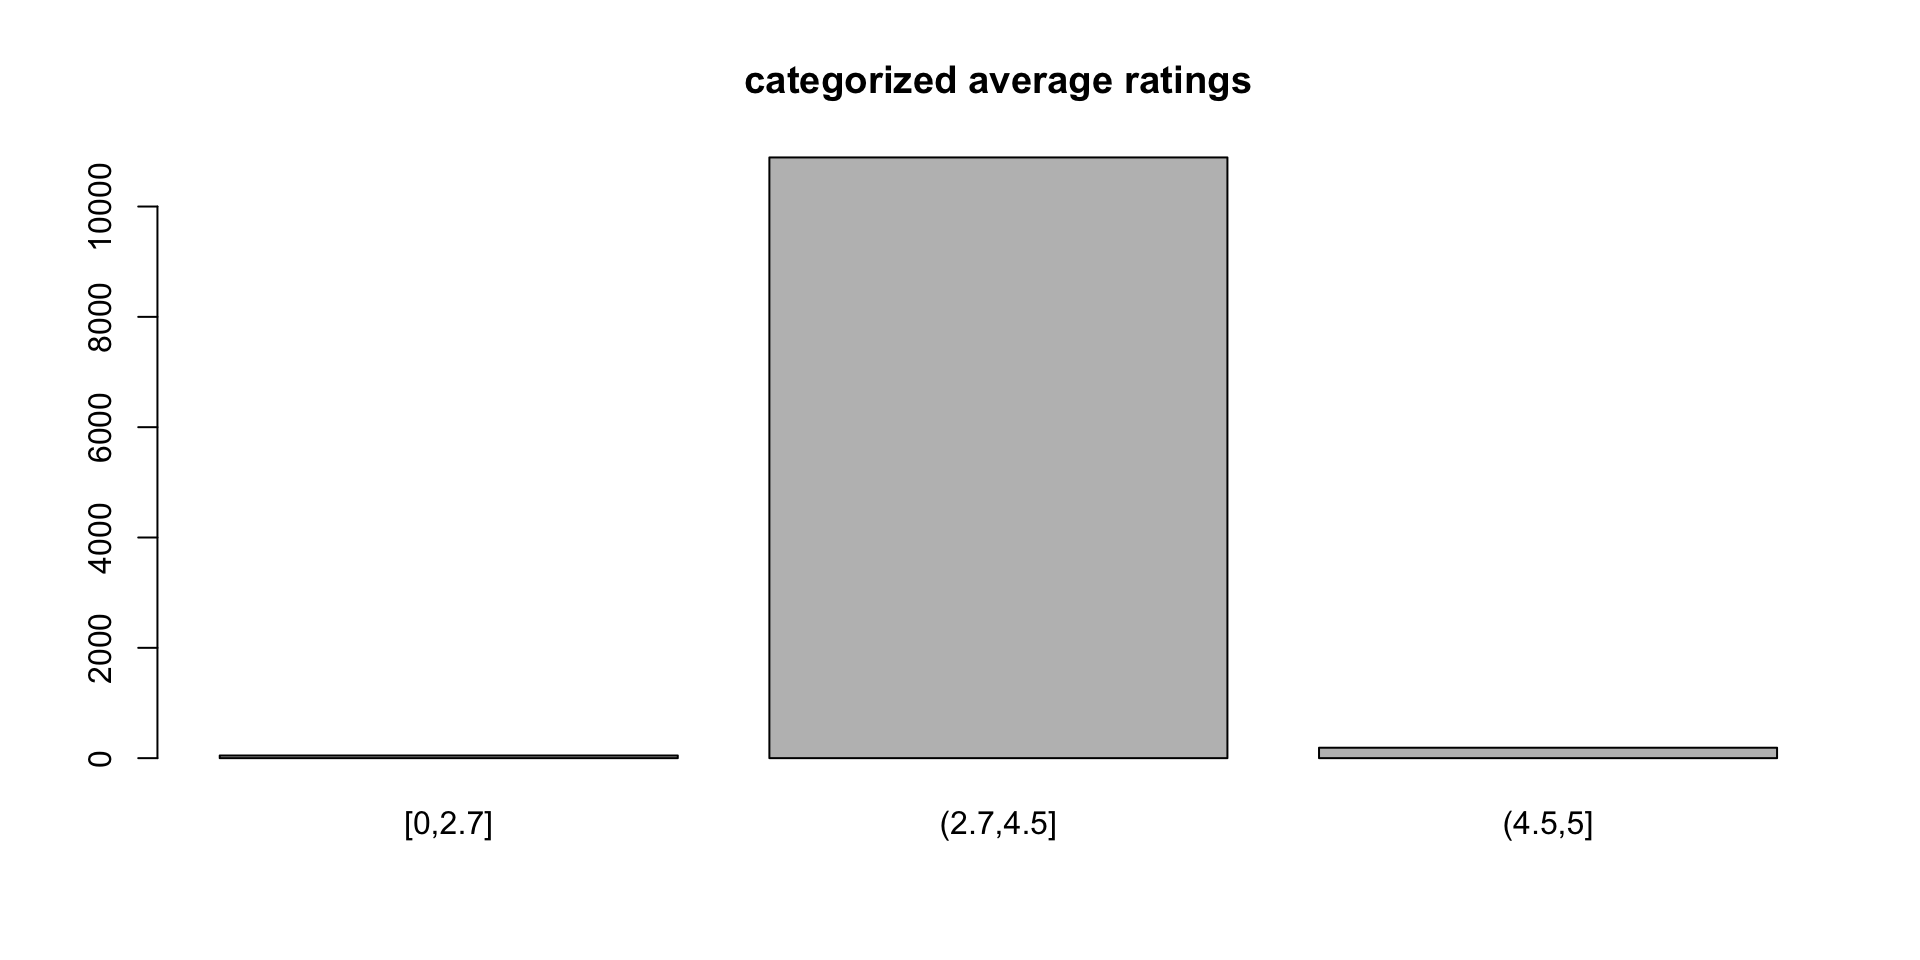
\includegraphics{Books_ratings_files/figure-latex/categorizing_average_ratings-1.pdf}

\begin{verbatim}
##   [0,2.7] (2.7,4.5]   (4.5,5] 
##        48     10890       189
\end{verbatim}

discretizing average rating turn it heavily unbalanced.

\begin{verbatim}
## av_cat
##   [0,2.7] (2.7,4.5]   (4.5,5] 
##      0.00      0.98      0.02
\end{verbatim}

Above 98\% of average rating are between 2.7 and 4.5.

analysis of categorical variable

\begin{verbatim}
## # A tibble: 6 x 7
##   title                             authors isbn  isbn13 langu~1 publi~2 publi~3
##   <chr>                             <chr>   <chr> <chr>  <chr>   <chr>   <chr>  
## 1 "Harry Potter and the Half-Blood~ J.K. R~ 0439~ 97804~ eng     9/16/2~ Schola~
## 2 "Harry Potter and the Order of t~ J.K. R~ 0439~ 97804~ eng     9/1/20~ Schola~
## 3 "Harry Potter and the Chamber of~ J.K. R~ 0439~ 97804~ eng     11/1/2~ Schola~
## 4 "Harry Potter and the Prisoner o~ J.K. R~ 0439~ 97804~ eng     5/1/20~ Schola~
## 5 "Harry Potter Boxed Set  Books 1~ J.K. R~ 0439~ 97804~ eng     9/13/2~ Schola~
## 6 "Unauthorized Harry Potter Book ~ W. Fre~ 0976~ 97809~ en-US   4/26/2~ Nimble~
## # ... with abbreviated variable names 1: language_code, 2: publication_date,
## #   3: publisher
\end{verbatim}

number of unique title

\begin{verbatim}
## [1] 10352
\end{verbatim}

what are the 5 most rated titles?

\begin{verbatim}
## # A tibble: 5 x 2
## # Groups:   title [5]
##   title                                                                  avera~1
##   <chr>                                                                    <dbl>
## 1 Comoediae 1: Acharenses/Equites/Nubes/Vespae/Pax/Aves                        5
## 2 Willem de Kooning: Late Paintings                                            5
## 3 Literature Circle Guide: Bridge to Terabithia: Everything You Need Fo~       5
## 4 Middlesex Borough (Images of America: New Jersey)                            5
## 5 Zone of the Enders: The 2nd Runner Official Strategy Guide                   5
## # ... with abbreviated variable name 1: average_rating
\end{verbatim}

number of unique authors

\begin{verbatim}
## [1] 6643
\end{verbatim}

Who are the five authors with high rated books ?

\begin{verbatim}
## # A tibble: 5 x 2
##   authors                                          mean_avg_rating
##   <chr>                                                      <dbl>
## 1 Aristophanes/F.W. Hall/W.M. Geldart                            5
## 2 Chris    Green/Chris Wright/Paul Douglas Gardner               5
## 3 Dennis Adler/R.L. Wilson                                       5
## 4 Elena N. Mahlow                                                5
## 5 Ian        Martin/Katie Elliott                                5
\end{verbatim}

Which are the 5 languages that occur the most ?

\begin{verbatim}
## # A tibble: 5 x 2
##   language_code num_books_published
##   <chr>                       <int>
## 1 eng                          8911
## 2 en-US                        1409
## 3 spa                           218
## 4 en-GB                         214
## 5 fre                           144
\end{verbatim}

What are the 5 publishers with most high rated books ?

\begin{verbatim}
## # A tibble: 5 x 2
##   publisher           mean_avg_rating
##   <chr>                         <dbl>
## 1 Academica Press                   5
## 2 Boosey & Hawkes Inc               5
## 3 Chartwell Books                   5
## 4 Courage Books                     5
## 5 Raintree                          5
\end{verbatim}

Academia press is the most productive publisher.

Which year displays the highest number of book published ? check date
format

cleaning publication date first

\begin{verbatim}
## [1] "11/31/2000" "6/31/1982"
\end{verbatim}

clean publication date

\begin{verbatim}
## [1] "9-16-2006" "9-1-2004"  "11-1-2003" "5-1-2004"  "9-13-2004" "4-26-2005"
\end{verbatim}

\begin{verbatim}
## [1] "2-1-1994"   "12-21-2004" "12-1-1988"  "8-1-1993"   "2-27-2007" 
## [6] "5-28-2006"
\end{verbatim}

\includegraphics{Books_ratings_files/figure-latex/hist year1-1.pdf}

\includegraphics{Books_ratings_files/figure-latex/hist year 2-1.pdf}

\begin{verbatim}
##    Min. 1st Qu.  Median    Mean 3rd Qu.    Max. 
##    1900    1998    2003    2000    2005    2020
\end{verbatim}

in this record, 75\% of books have been published by 2005.

\begin{verbatim}
## # A tibble: 5 x 2
##    year n_books_published
##   <dbl>             <int>
## 1  2006              1700
## 2  2005              1260
## 3  2004              1071
## 4  2003               931
## 5  2002               798
\end{verbatim}

Year 2006 , yields 1700 books published.

2D EDA

\end{document}
